\documentclass{report}
\usepackage[T1]{fontenc} % Fontes T1
\usepackage[utf8]{inputenc} % Input UTF8
\usepackage{csquotes}
\usepackage[portuguese]{babel} %Usar língua portuguesa
\usepackage{blindtext} % Gerar texto automaticamente
\usepackage[printonlyused]{acronym}
\usepackage{hyperref} % para autoreferencia
\usepackage{graphicx}
\usepackage{float}
\usepackage{subcaption}
\usepackage{makeidx}
\usepackage[backend=biber, style=ieee]{biblatex} % para usar bibliografia

\addbibresource{biblatex-examples.bib}

\begin{document}
%%
% Definições
%
\def\titulo{Projeto 2}
\def\data{14/06/2019}
\def\autores{Luís Couto, Francisco Silva, Joaquim Andrade}
\def\autorescontactos{(89078), (93400), (93432) }
\def\versao{1}
\def\departamento{\acs{deti}}
\def\empresa{Universidade de Aveiro}
\def\logotipo{ua.pdf}
\def\projeto{\href{https://code.ua.pt/projects/labi2019-p2-g19}{labi2019-p2-g19}}

%
%%%%%% CAPA %%%%%%
%
\begin{titlepage}

\begin{center}
%
\vspace*{50mm}
%
{\Huge \titulo}\\ 
%
\vspace{10mm}
%
{\Large \empresa}\\
%
\vspace{10mm}
%
{\LARGE \autores}\\ 
%
\vspace{30mm}
%
\begin{figure}[h]
\center
\includegraphics{\logotipo}
\end{figure}
%
\vspace{30mm}
\end{center}
%
\begin{flushright}
\versao
\end{flushright}
\end{titlepage}


%%  Página de Título %%
\title{%
{\Huge\textbf{\titulo}}\\
{\Large \departamento\\ \empresa}
}
%
\author{%
    \autores \\
    \autorescontactos \\
    \projeto 
}
%
\date{\data}
%
\maketitle

\pagenumbering{roman}
 
\begin{abstract}
\begin{large}
\paragraph{}
Seja no facebook, seja no instagram, ou até nas nossas próprias câmaras de telemóvel, é possível ver que existe um reconhecimento facial automático. O reconhecimento não só facial mas também como de outros objetos em imagens, vídeos e até mesmo na vida real é um tema muito atual e alvo de muita pesquisa e foco científico.
\paragraph{}
Este trabalho vai ao encontro desse tema, pois tem como objetivo desenvolver uma Aplicação Web, que fazendo uso de um site capaz de reconhecer objetos em imagems\cite{Object_Detection}, permita tratar essas imagens, guardá-las numa base de dados e fazer várias pesquisas com elas.
Neste relatório falaremos da Aplicação Web que desenvolvemos, do código que fizemos para a Interface Web, da maneira que implementámos o processador de imagens e o tipo de base de dados que criámos. 
\paragraph{}
Iremos falar de cada módulo desenvolvido, assim como apresentaremos imagens que demonstram o funcionamento correto do código desenvolvido.
No final iremos analisar os resultados e tirar conclusões.
\end{large}
\end{abstract} 
 
\tableofcontents

\listoffigures

\chapter*{Acrónimos}
\begin{acronym}
\acro{deti}[DETI]{- Departamento de Electrónica, Telecomunicações e Informática}
\acro{li}[LI]{- Laboratórios de Informática}
\end{acronym}

%%%%%%%%%%%%%%%%%%%%%%%%%%%%%%%% CAPITULO 1 - INTRODUÇÃO
\chapter{Introdução}
\label{chap.introducao}
\large
\section{Motivação e Objetivos}
\paragraph{}
No âmbito da avaliação da cadeira de \acs{li}, foi-nos proposto efetuar um projeto que aplicava todos os conhecimentos adquiridos ao longo dos dois semestres da cadeira (\textit{Python}, HTML, CSS, JavaScript, entre outros) e que tinha como objetivo principal criar uma Aplicação Web.
\paragraph{}
O que era pedido desta Aplicação Web era que fosse possivel carregar imagens para o sistema, que depois iriam ser reencaminhadas para o site fornecido no guião\cite{Object_Detection}. Este site iria devolver um ficheiro JSON com os diversos objetos presente na imagem, incluindo as coordenadas necessárias para recortar cada um dos objetos e a confiança. Este ficheiro iria depois ser usado pelo processador para fazer o respetivo tratamento de imagem. Estas imagens e objetos iriam depois ficar guardados numa base de dados, sendo possível ao utilizador fazer pesquisas sobre eles de várias maneiras.

\section{Conteúdo disponibilizado}
\paragraph{}
Quanto ao trabalho, existem 2 pastas, cada uma com o seguinte conteúdo:
\begin{enumerate}
	\item codigo
    \begin{enumerate}
    	\item Interface (ficheiros necessário para o website)
    	\item Original (imagens originais)
        \item Objects (objetos recortados das imagens originais)
        \item images.db (base de dados)
        \item processador.py (ficheiro com as funções para tratar as imagens)
        \item main.py (ficheiro CherryPy que é a aplicação)
    \end{enumerate}
    \item relatorio
    \begin{enumerate}
    	\item TrabalhoP2.pdf
        \item Todas as imagens usadas
        \item Todos os ficheiros fonte necessários
    \end{enumerate}
\end{enumerate}
\paragraph{}
Quando a este relatório, está dividido em 6 capítulos. Depois desta introdução, no \autoref{chap.interface} falamos da implementação da Interface Web e como navegar pelo website. No \autoref{chap.processador} é esclarecido o algoritmo do processador de imagens, sendo apresentada uma explicação detalhada e imagens dos resultados. \newline
No \autoref{chap.BD} é feita uma breve referência à base de dados criada, no \autoref{chap.aplicação} é falado na Aplicação Web e sendo que por fim, no \autoref{chap:conclusao}, são tiradas conclusões.

%%%%%%%%%%%%%%%%%%%%%%%%%%%%%%%% CAPITULO 2 - INTERFACE

\chapter{Interface Web}
\label{chap.interface}

\section{Estrutura da Interface}
Para a implementação da Interface Web, foi usado um \textit{template} \textit{bootstrap}\cite{Template_Bootstrap} como base fundamental, no entanto foram feitas alterações a nível de código, de estrutura e de \textit{display} do website. 

\section{Página Inicial}
\paragraph{}

\begin{figure}[H]
\centering
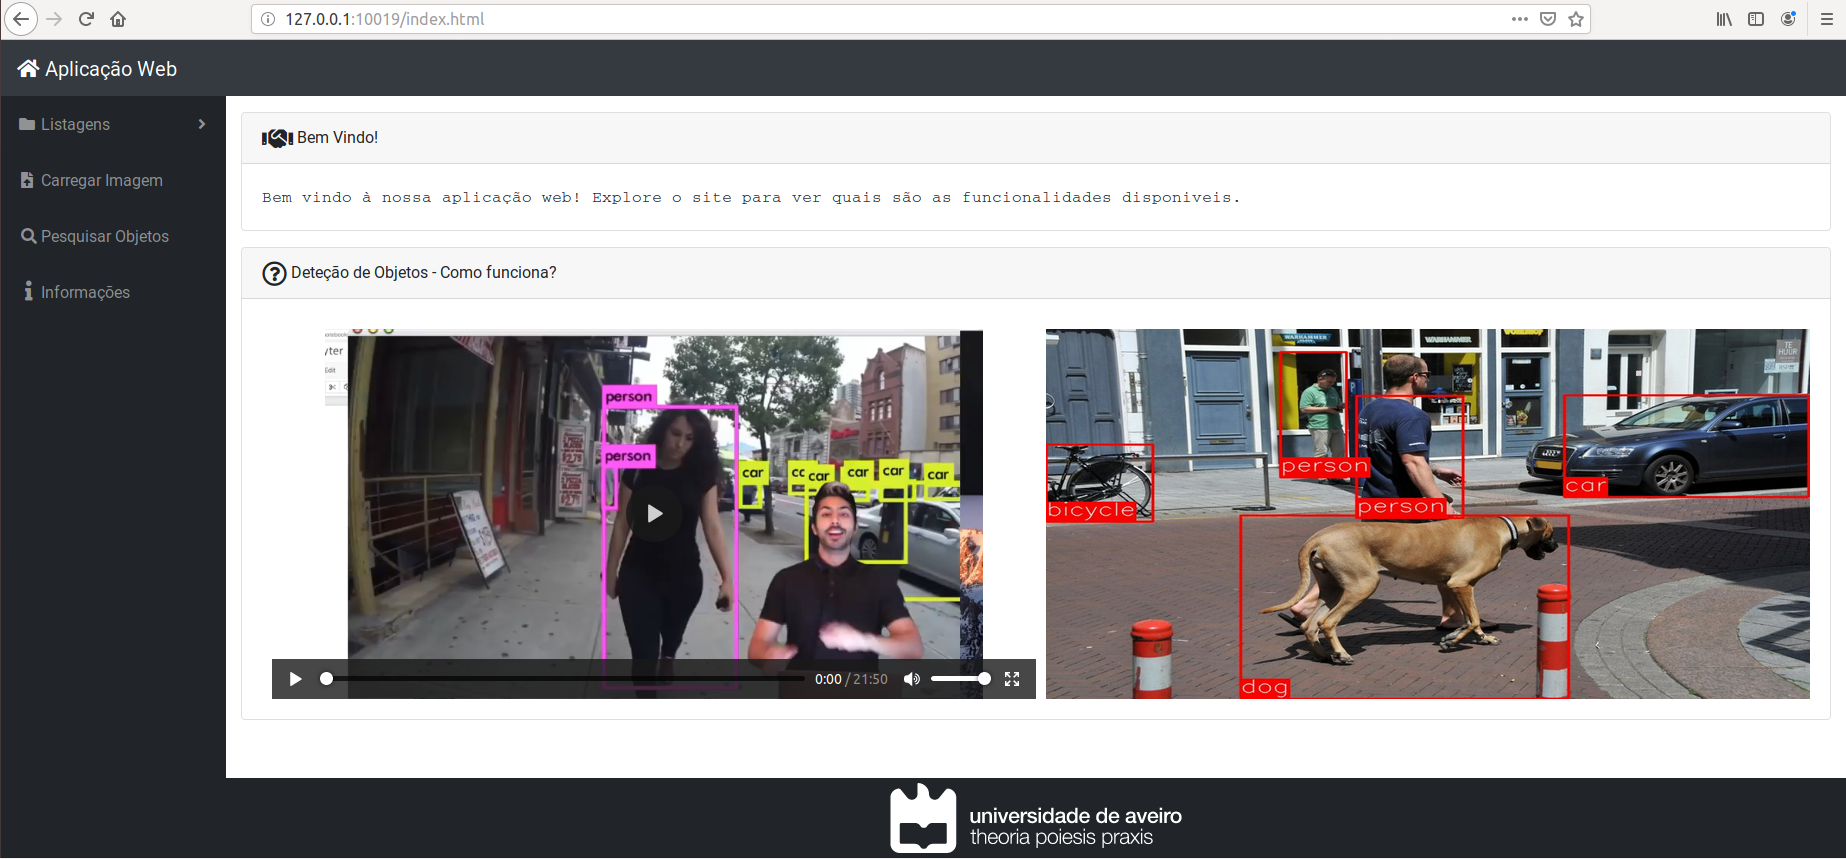
\includegraphics[width=1\linewidth]{index.png}
\caption{index.html}
\end{figure}

Esta é a página inicial do website. O utilizador pode ver um vídeo informativo sobre a deteção de objetos ou então pode navegar para outras páginas usando a \textit{sidebar}.


\section{Listar Objetos}
\paragraph{}

\begin{figure}[H]
\centering
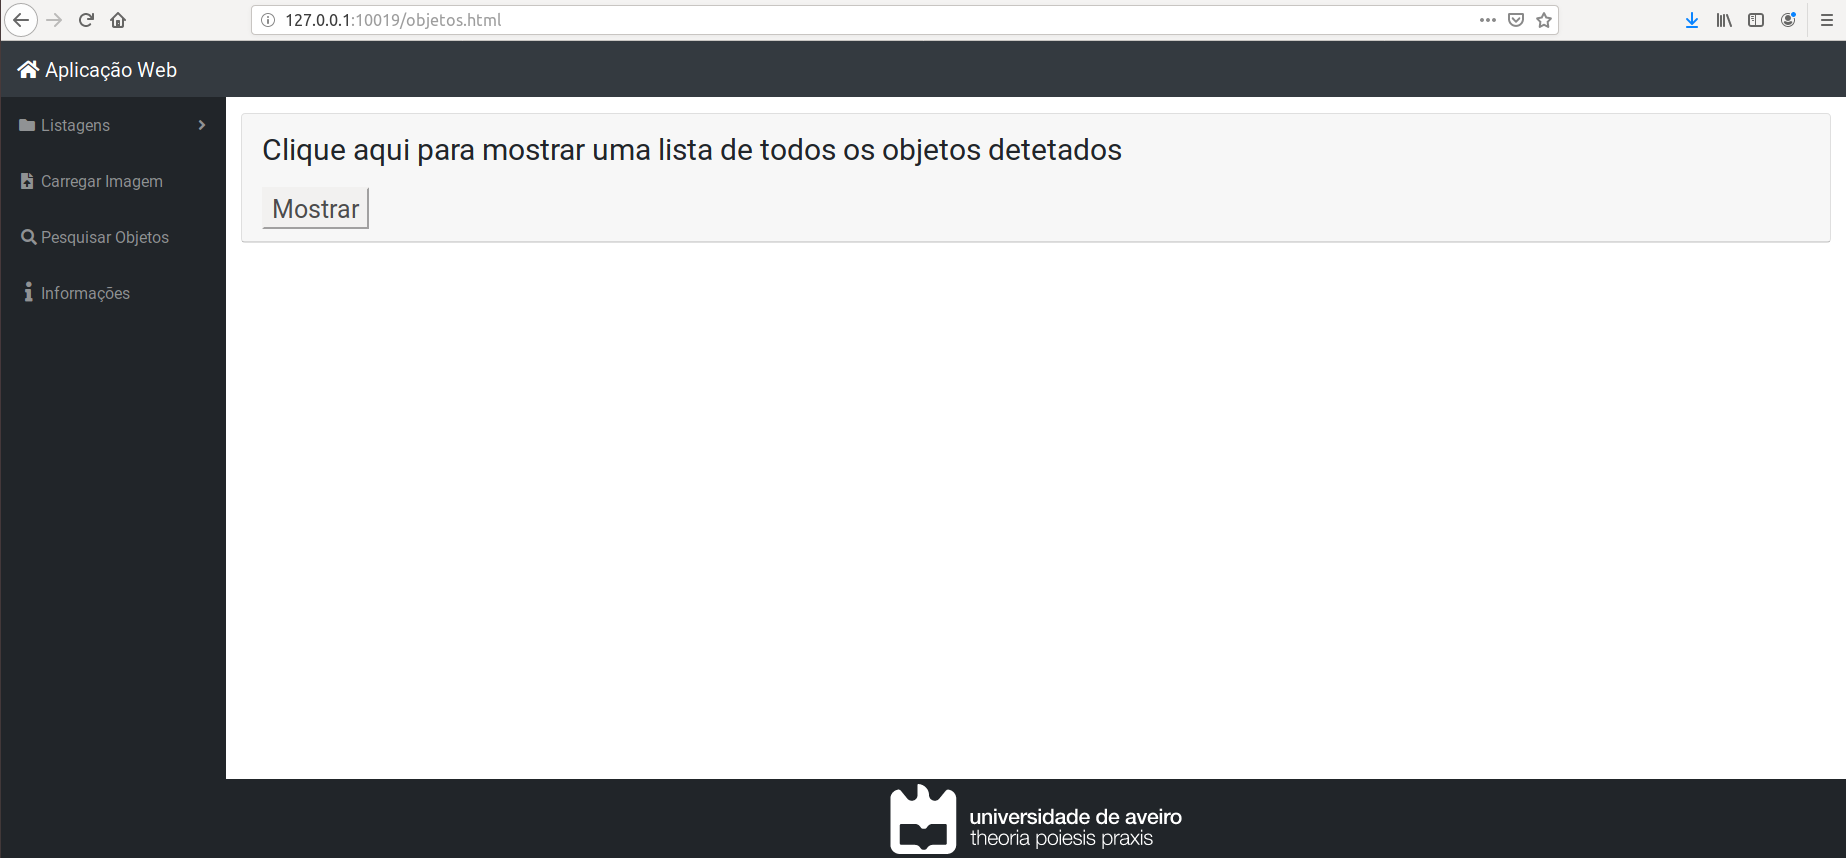
\includegraphics[width=1\linewidth]{objetos.png}
\caption{objetos.html}
\end{figure}

Nesta página, o utilizador pode listar todos os objetos que já foram detetados pressionando o botão indicado.


\section{Listar Imagens}
\paragraph{}

\begin{figure}[H]
\centering
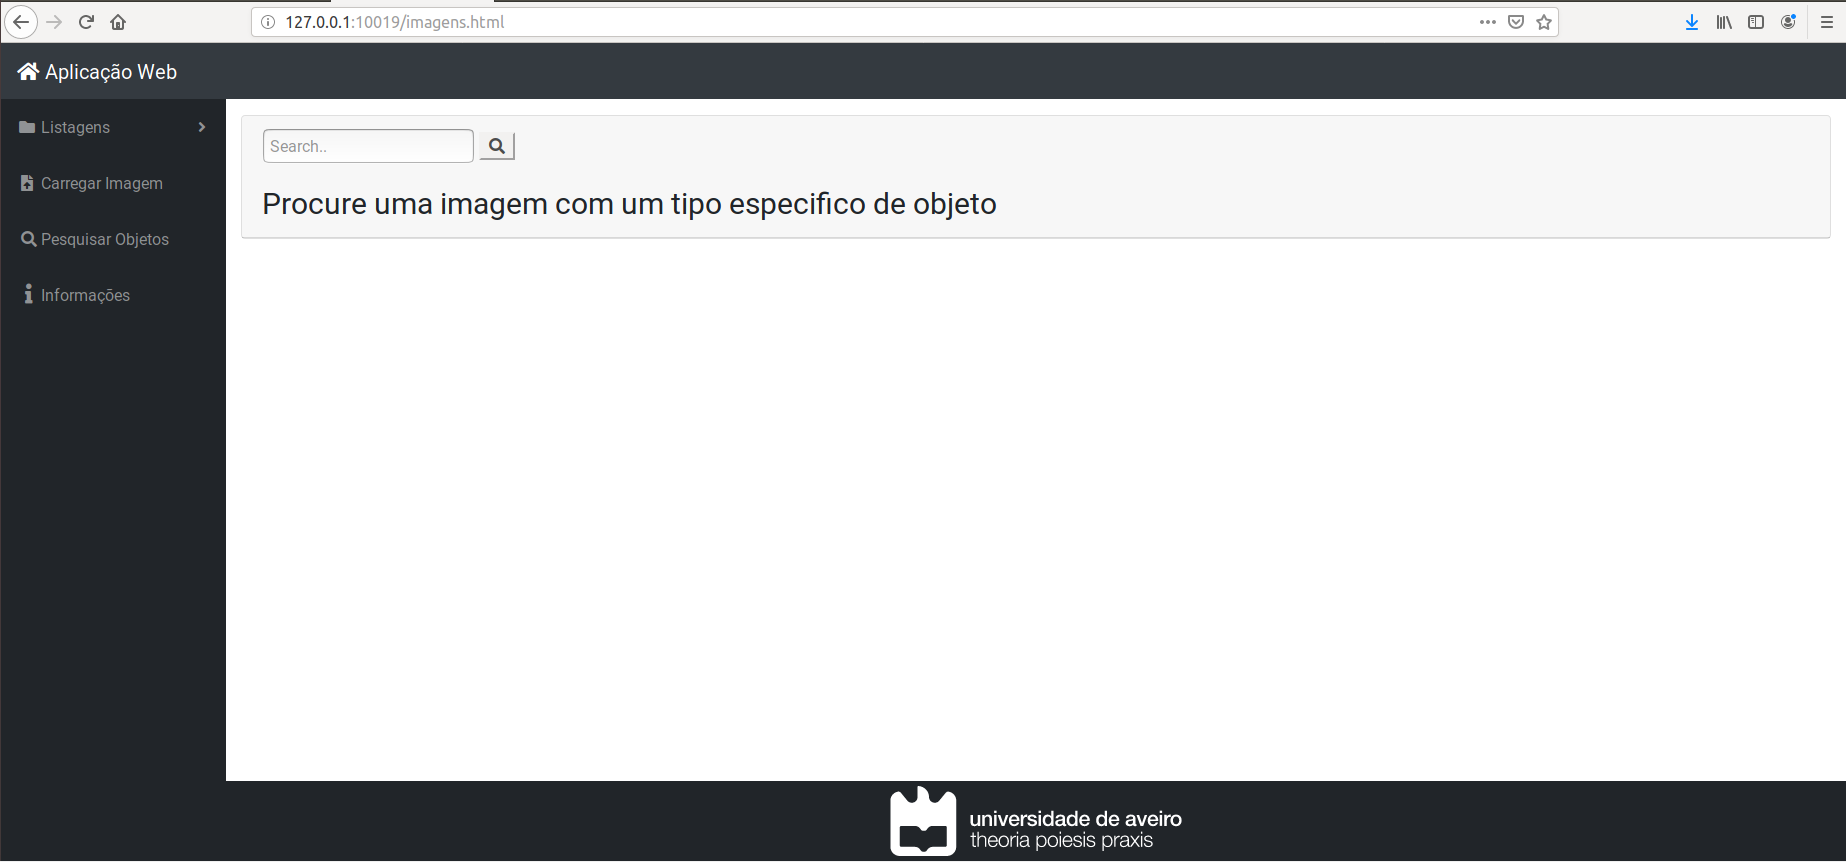
\includegraphics[width=1\linewidth]{imagens.png}
\caption{imagens.html}
\end{figure}

Nesta página, o utilizador pode procurar por um determinado objeto (car, person,...). O website vai então mostrar todas imagens que contenham esse objeto, com um limiar de confiança de 50.


\section{Carregar Imagem}
\paragraph{}

\begin{figure}[H]
\centering
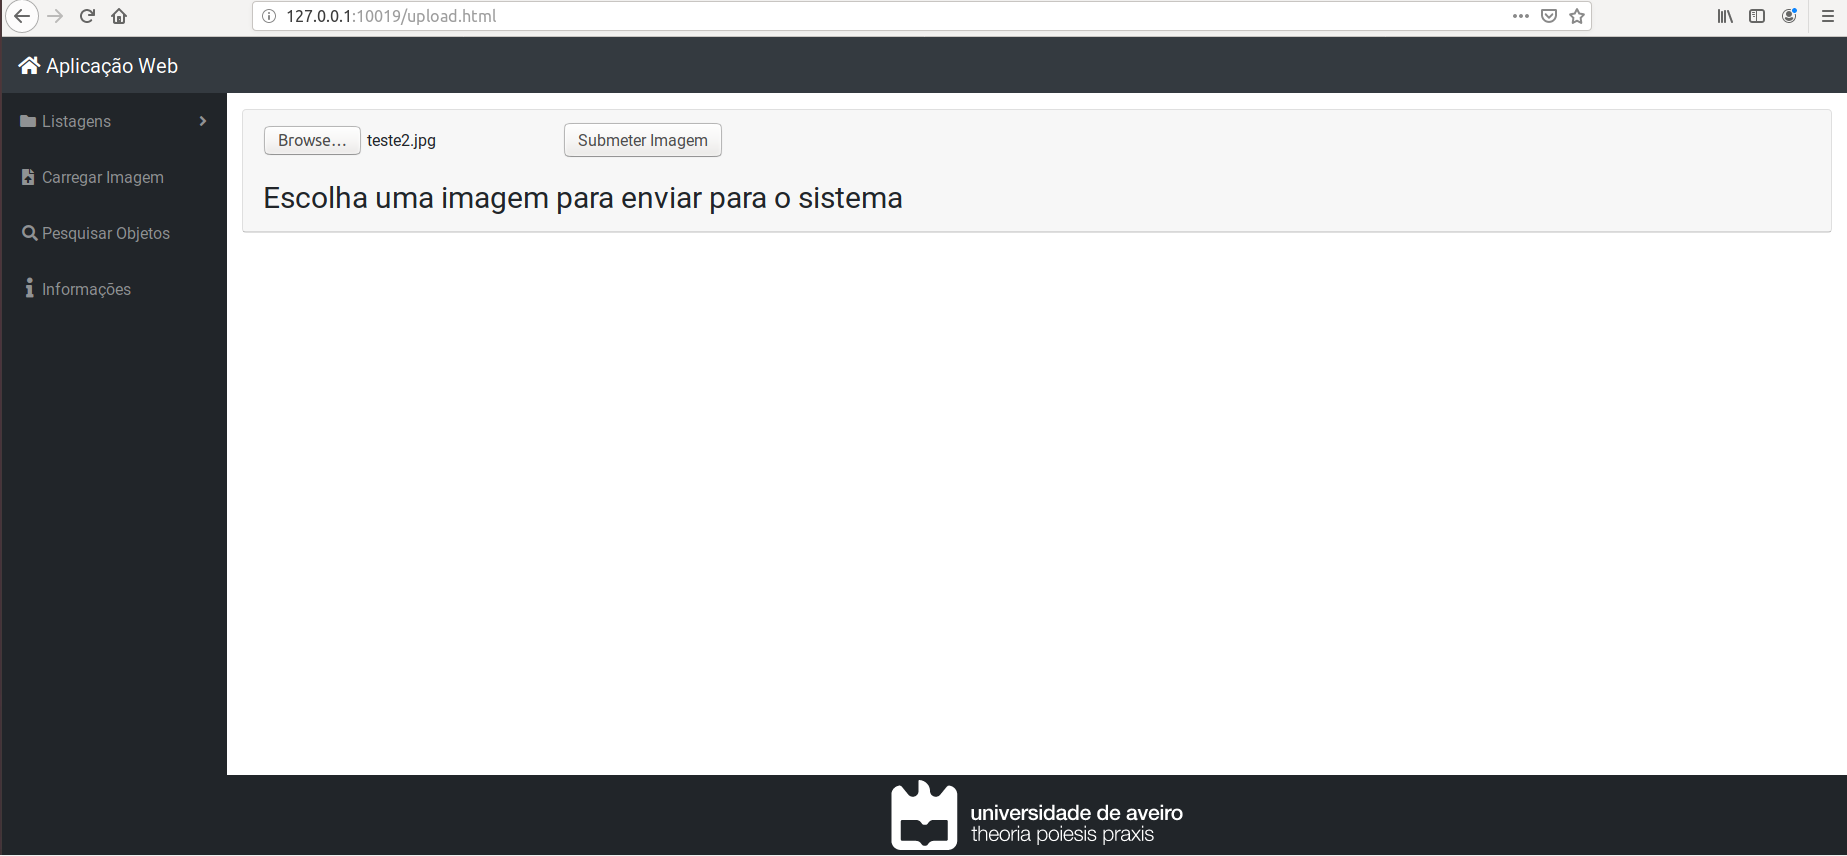
\includegraphics[width=1\linewidth]{upload.png}
\caption{upload.html}
\end{figure}

Nesta página, o utilizador pode enviar qualquer imagem para o sistema. Esta imagem vai depois ser tratada segundo as especificações pedidas e guardada na base de dados, assim como qualquer objeto recortado a partir desta.


\section{Pesquisar Objetos}
\paragraph{}

\begin{figure}[H]
\centering
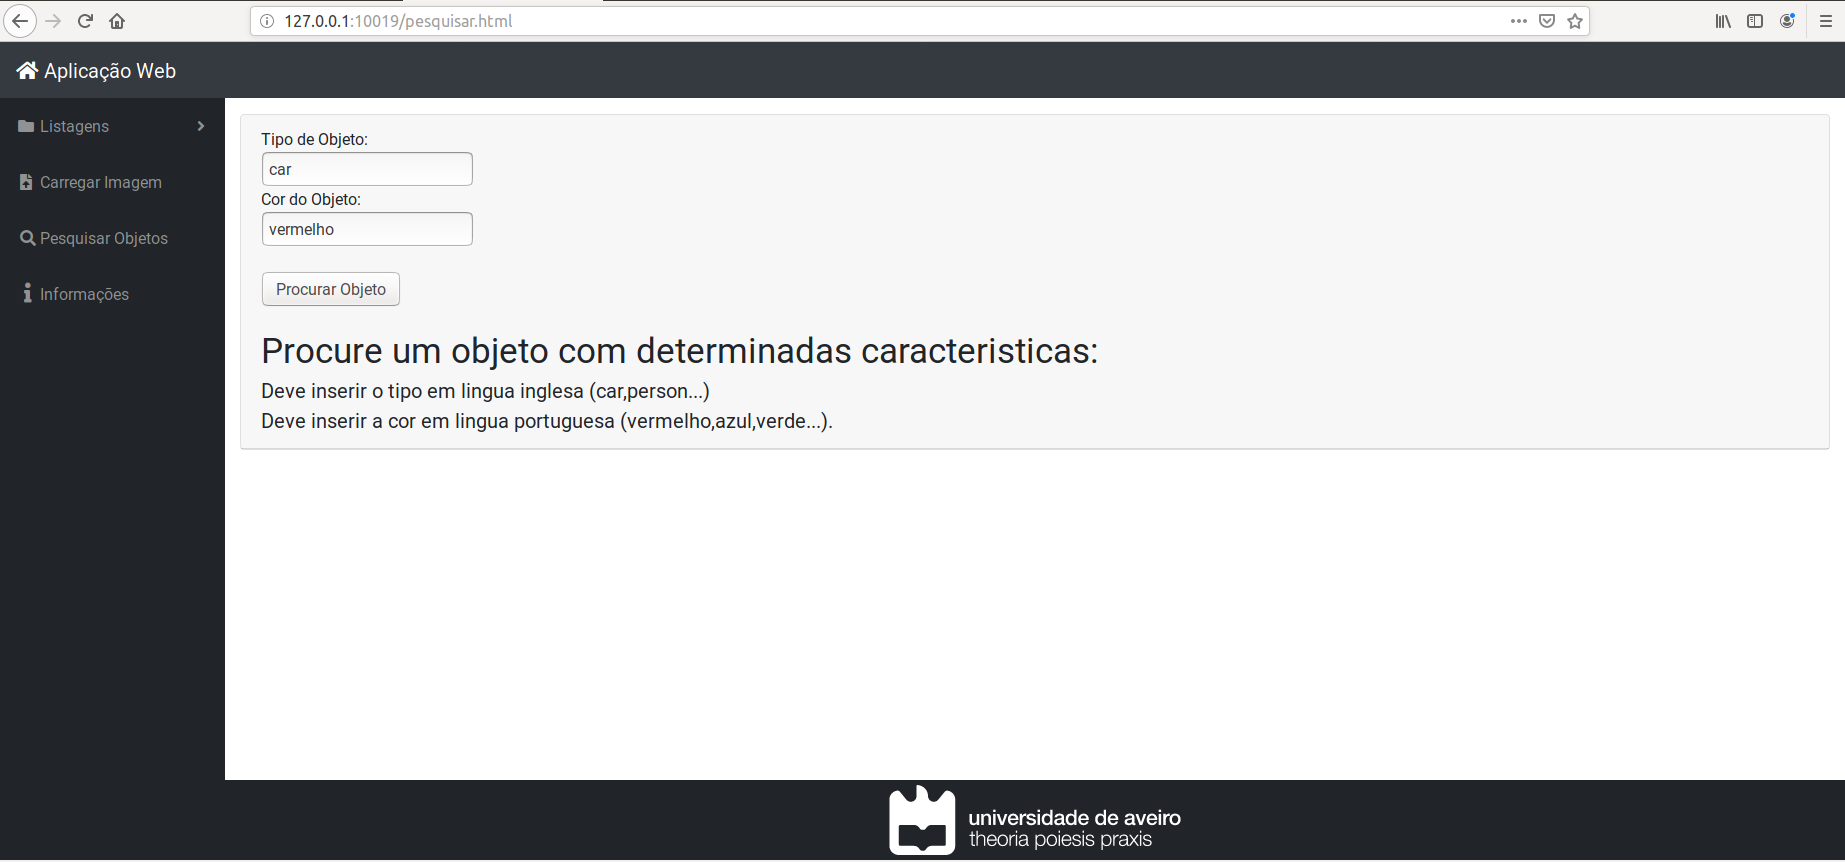
\includegraphics[width=1\linewidth]{pesquisar.png}
\caption{pesquisar.html}
\end{figure}

Nesta página, o utilizador pode procurar por um determinado objeto (car, person,...) com uma determinada cor (vermelho,verde,azul,..). Devido à maneira como a nossa base de dados está feita, o objeto tem de ser un input em inglês e a cor um input em português.



\section{Informações}
\paragraph{}

\begin{figure}[H]
\centering
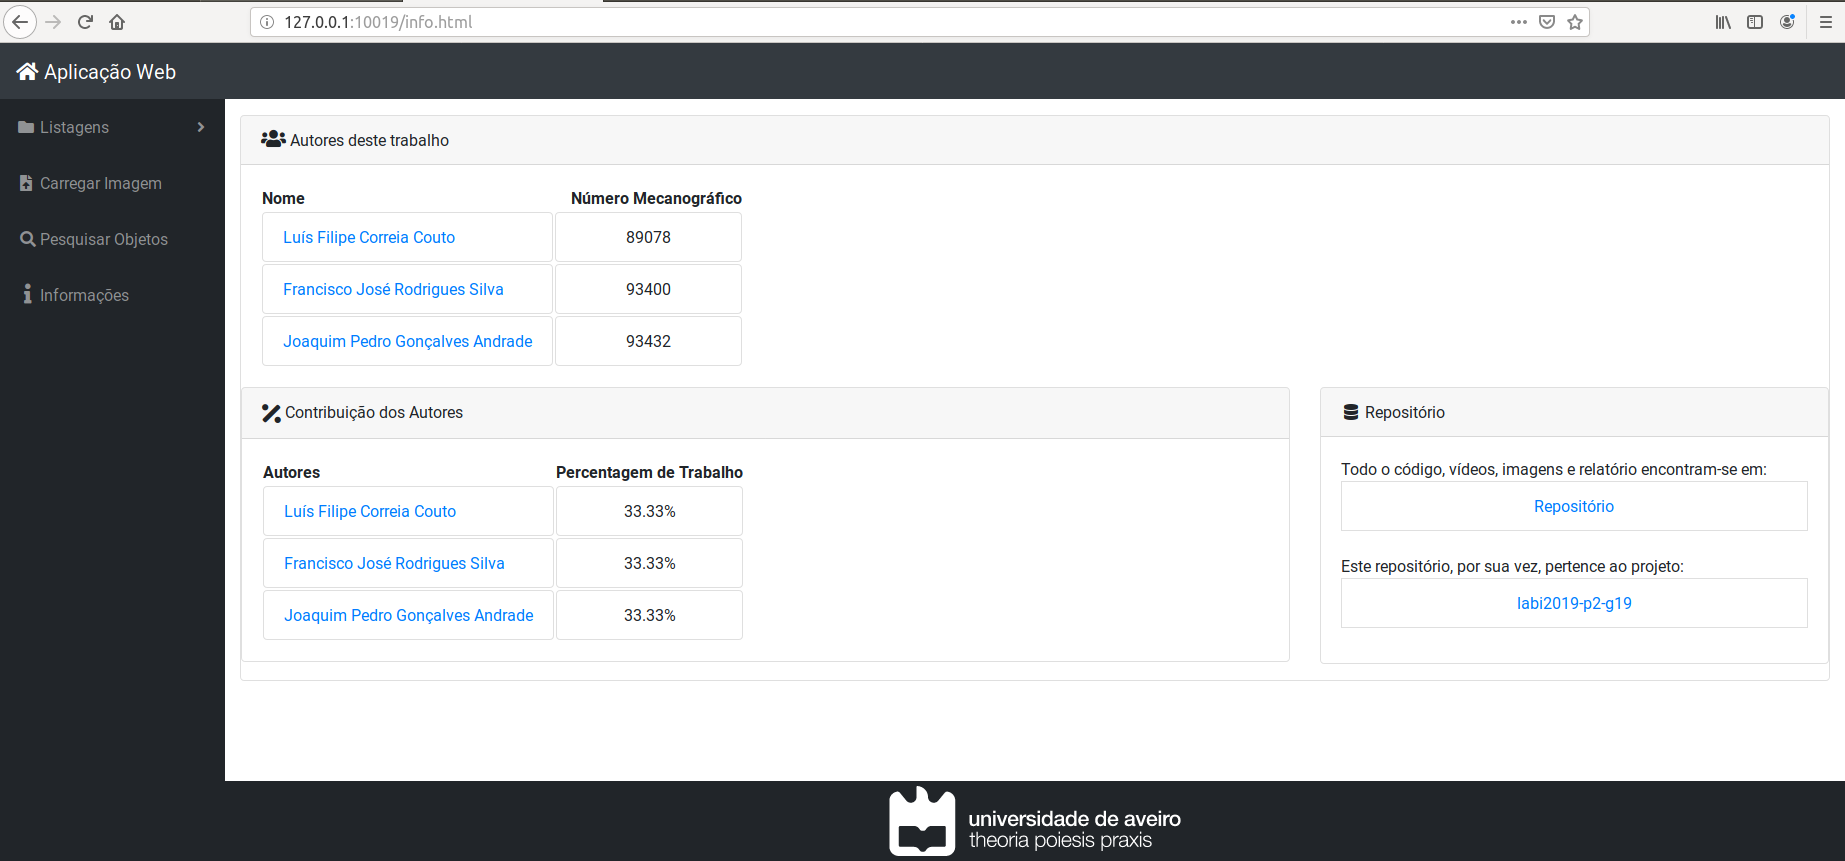
\includegraphics[width=1\linewidth]{info.png}
\caption{info.html}
\end{figure}

Nesta página, o utilizador pode ler informação sobre os autores, a sua contribuição ou o repositório onde o código do projeto se encontra.



%%%%%%%%%%%%%%%%%%%%%%%%%%%%%%%% CAPITULO 3 - IMPLEMENTAÇÃO DO PROCESSADOR

\chapter{Processador de Imagens}
\label{chap.processador}
\paragraph{}
Neste capítulo vai ser explicada a implementação do processador de imagens, que se encontra implementado no ficheiro processador.py.
Devido a extensão do código não vamos por imagens dele neste relatório, no entanto vamos fazer uma descrição detalhada e mostrar resultados ao fim de dar \textit{run} a este programa usando uma imagem.


\section{Implementação}
\paragraph{}
O processador de imagens é um programa em \textit{python} que recebe uma imagem enviada e
efetua várias operações com ela. 

\paragraph{}

Em primeiro lugar, fazendo uso do módulo “requests”, o programa envia a imagem para o URL
disponibilizado no guião\cite{Object_Detection} e guarda numa variável o ficheiro json que é devolvido. 
\paragraph{}
O ficheiro json contém informações sobre os objetos identificados pelo serviço, como a
class (tipo de objeto), coordenadas (x, y, x1, y1) que representam uma caixa de identificação dos objetos
que foram encontrados e identificados e um valor de confiança que é a confiança que o serviço
tem de que identificou um objeto e a sua class corretamente. 
\paragraph{}
Em segundo lugar o programa utiliza as coordenadas devolvidas pelo serviço e cria novas
imagens com um recorte das imagens originais, um para cada objeto encontrado. A função
\textbf{creatbox} guarda os valores da class, confiança e guarda num \textit{tuple} as coordenadas,
representando uma caixa que vai ser usada para o recorte das imagens e devolve todas estas
informações. 
\paragraph{}
Com a função \textbf{crop} do módulo Image que recebe como argumento um \textit{tuple} com as coordenadas,
é feito o recorte dos objetos encontrados na imagem original. As imagens geradas dos objetos
identificados são então guardadas num diretório à parte (pasta \textbf{Objects)}, tal como as imagens originais(pasta \textbf{Original}.
\\
Numa terceira fase o programa analisa cada uma das imagens que representam os objetos
encontrados e tenta classificar o objeto com uma cor. Nesta classificação considerámos as
cores: vermelho, laranja, amarelo, verde, azul, violeta, preto, branco e cinzento. \linebreak
\paragraph{}
Para a implementação do problema das cores considerámos cada pixel da imagem como uma
combinação das cores vermelho, verde e azul. Podemos saber os valores de RGB usados em
cada pixel da imagem e usámos isso para classificar cada um dos pixéis com uma cor.
\\
Considerámos limites de representação para cada um dos canais RGB. Num pixel uma cor com
valor menor que o limite inferior(85) é classificado como baixo, com valor maior que o
limite superior(170) é classificado como alto e caso esteja dentro dos limites é classificado
como médio. 
\paragraph{}
Destas combinações de cores e classificações tivemos de considerar $(3^3) = 27$ possibilidades e
atribuir uma cor a cada uma. Classificado cada pixel, basta fazer a contagem, e a cor associada
ao maior número de pixéis é considerada a cor dominante na imagem.
Face a alguns problemas que encontrámos na implementação desta solução decidimos criar
um filtro que funciona como uma variável booleana e que limita a cor preta. 
\paragraph{}
Face aos limites que considerámos a cor preta era considerada dominante na maioria das imagens visto que
algumas cores próximas do preto e presentes em várias imagens eram classificadas como
preto adulterando de certa forma os resultados. 
\paragraph{}
Calculada a cor temos todas as informações que precisamos e o programa procede.


\section{Resultados}
\paragraph{}
Ao corrermos este código com uma imagem original que contenha vários objetos, obtemos o seguinte resultado.

\begin{figure}[H]
\centering
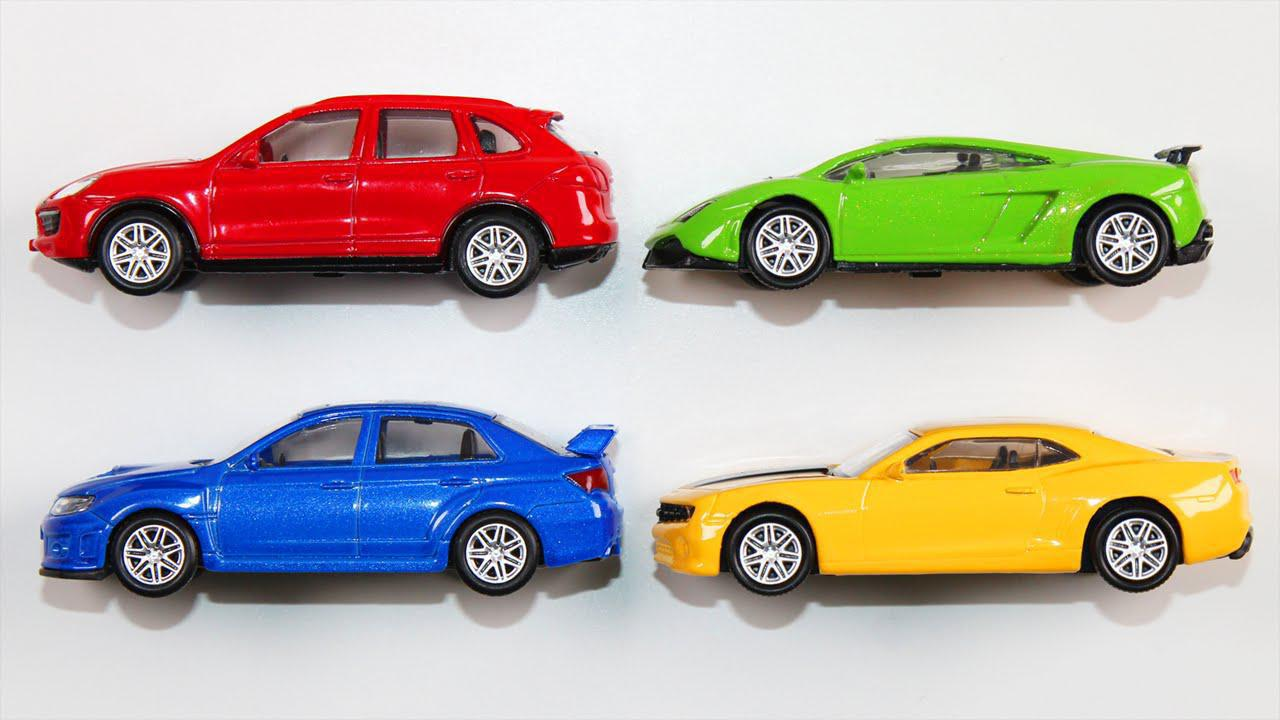
\includegraphics[width=0.75\linewidth]{teste.jpg}
\caption{Imagem para testar processador}
\end{figure}


\begin{figure}[H]
\centering
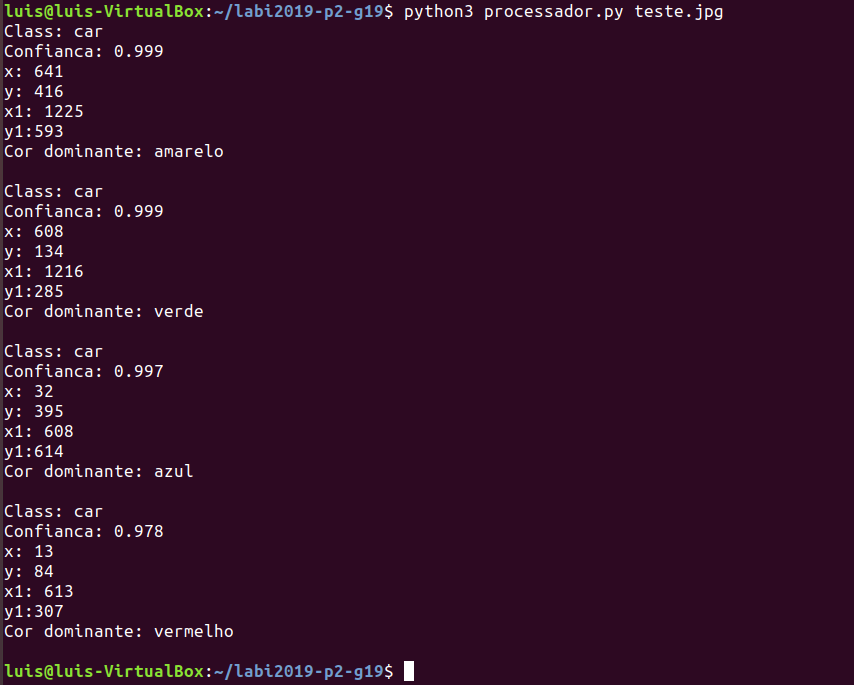
\includegraphics[width=0.75\linewidth]{consola.png}
\caption{Resultado impresso na consola}
\end{figure}


\begin{figure}[H]
\centering
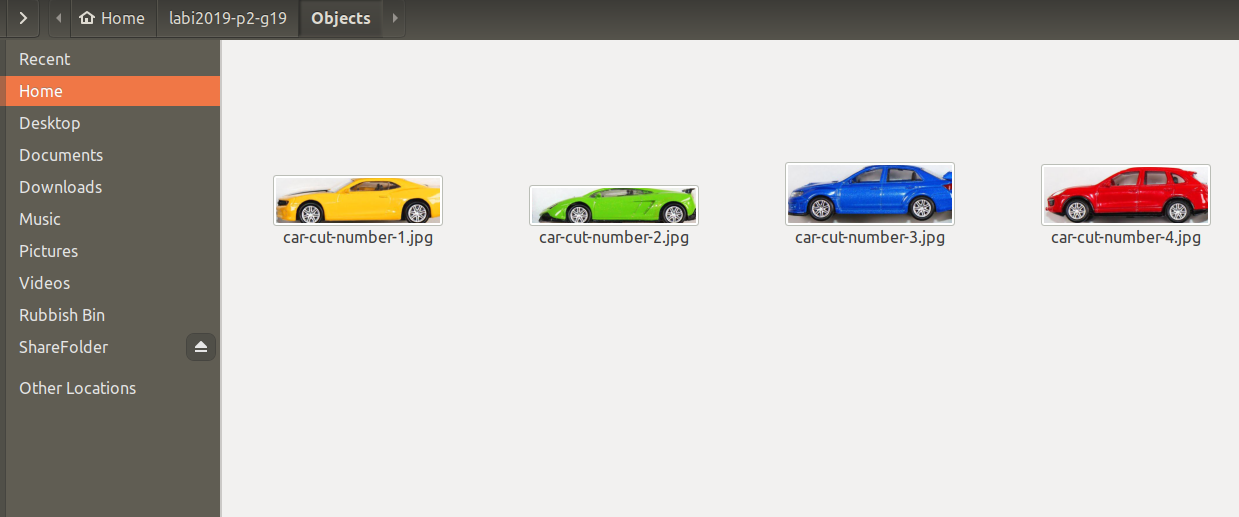
\includegraphics[width=1.3\linewidth]{carros.png}
\caption{Objetos recortados pelo processador a partir da imagem original, guardados no respetivo diretório}
\end{figure}


\chapter{Base de Dados}
\label{chap.BD}
\paragraph{}

A primeira tabela é referente às imagens originais. Contém 4 campos que são o \textbf{id} que incrementa automáticamente à medida que vão sendo introduzido dados, o \textbf{nome} da imagem, a \textbf{síntese} que é a síntese (SHA-512) da imagem original e o \textbf{path} que contém o caminho do diretório onde a imagem está armazenada.

\paragraph{}

A segunda tabela é referente às imagens que contém objetos recortados a partir das imagens originais. Contém 11 campos que são o \textbf{input\_id} que incrementa automáticamente à medida que vão sendo introduzido dados, a \textbf{class} que é o tipo de objeto detetado, a \textbf{var\_x}, \textbf{var\_y}, \textbf{var\_x1} e \textbf{var\_y1} que são as coordenadas de uma caixa na imagem original onde se encontra o objeto, a \textbf{confidence} que é a confiança, o \textbf{sha\_original} que é a síntese (SHA-512) da imagem original, o \textbf{sha\_objeto} que é a sintese (SHA-512) da imagem que contém o objeto recortado, a \textbf{cor} do objeto e o \textbf{path} que contém o caminho do diretório onde o objeto está armazenado.

\begin{figure}[H]
\centering
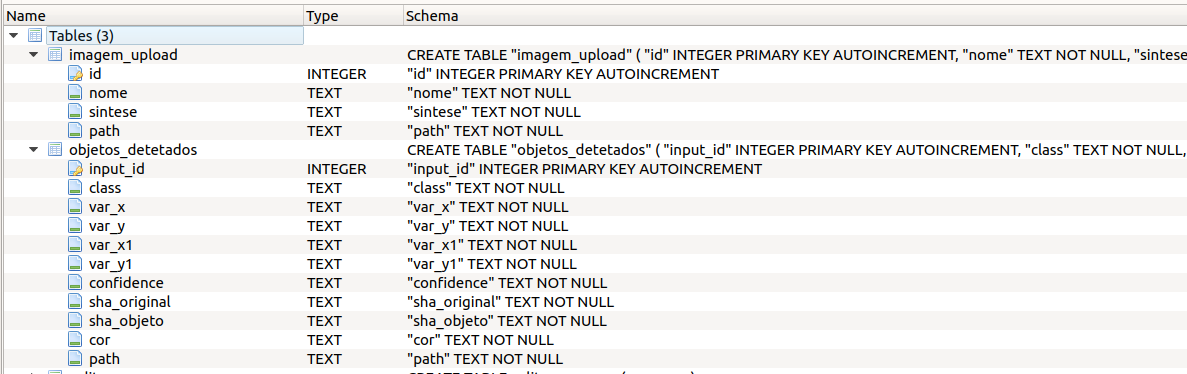
\includegraphics[width=1\linewidth]{db.png}
\caption{Base de Dados criada}
\end{figure}



\chapter{Aplicação Web}
\label{chap.aplicação}
\paragraph{}
A aplicação principal deste trabalho é o ficheiro \textbf{main.py}. Para iniciar a aplicação, o utilizador tem de correr na consola o ficheiro \textbf{main.py} e aceder ao endereço que aparece indicado na consola.


\begin{figure}[H]
\centering
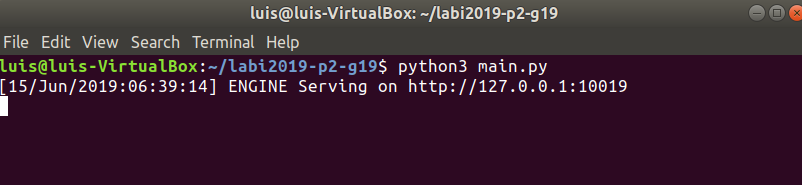
\includegraphics[width=1\linewidth]{app.png}
\caption{Iniciar a Aplicação}
\end{figure}

\paragraph{}
Para formarmos a aplicação web usamos então o módulo cherrypy em python. O cherrypy é um servidor aplicacional. Temos então a declaração de uma classe \textbf{Root}. Esta classe é composta por um método chamado \textbf{index}. 
\textbf{@cherrypy.expose} determina que o método \textbf{index} deverá ser exposto ao cliente Web. O método \textbf{index} devolve um html.
\paragraph{}
Após esse método temos o método \textbf{listnames} que se conecta à base de dados e devolve um objeto json com uma lista de todos os objetos já detectados.
Temos também o método \textbf{listdetected} que devolve um objeto json com as sínteses das imagens dos objetos cortados, juntamente com a imagem original e a confiança. Neste método foi aplicada a identação do objeto json de modo a que o resultado final seja de acordo com o pedido no guião.
Após este método temos dois métodos semelhantes, no entanto com filtros. Estes filtros foram aplicados através da alteração do comando execute da base de dados, que nos permitiu facilmente alcançá-los.
\paragraph{}
O método \textbf{put} por sua vez serve para inicializar uma nova imagem. Este processo leva-nos diretamente para o nosso processador de imagens. Este processador tem também vários métodos dos quais falaremos mais à frente. Este método envia no final, toda a informação requerida para a base de dados.
O método \textbf{identifier}, mais uma vez conecta-se à base de dados e procura, novamente, usando uma particularidade do execute, o caminho de uma imagem através da sua síntese.

\chapter{Conclusão:}
\label{chap:conclusao}
\paragraph{}	

Este foi um trabalho desafiante que pôs à prova todos os conhecimentos adquiridos ao longo do ano. Apesar de termos conseguidos fazer os blocos inviduais do trabalho e eles funcionarem, o produto final não é o esperado. Devido à menor dimensão do nosso grupo e consequente falta de tempo, não foi possível escrever código JavaScript, e sem este código não foi possível por a aplicação a funcionar como desejado, pois a Interface Web não comunica com o resto dos blocos.


\section{Contribuição dos autores}
\paragraph{}
O aluno Luís Couto ficou encarregue da Interface Web e base de dados. \\
O aluno Francisco Silva ficou encarregue do processador de imagens. \\
O aluno Joaquim Andrade ficou encarregue da Aplicação Web. 
\paragraph{}
O relatório foi escrito pelo aluno Luís Couto com a assistência dos outros dois membros.
\paragraph{}
Tendo isto em conta, a contribuição de cada aluno foi de 33.33 \%.
\paragraph{}
A área utilizada no XCOA é \href{https://xcoa.av.it.pt/labi2019-p2-g19}{https://xcoa.av.it.pt/labi2019-p2-g19}.
\\
A projeto no Code.UA é \href{https://code.ua.pt/projects/labi2019-p2-g19}{https://code.ua.pt/projects/labi2019-p2-g19}.
%%%%%%%%%%%%%%%ACABA

\printbibliography

\end{document}


